\chapter{Fourier Transform}
\section{Aliasing}
One can't shrink an image by taking every second pixel. If we do, characteristic errors appear. Typically, small phenomena look bigger; fast phenomena can look slower. Common phenomenons
\begin{inparaenum}[\itshape(1)]
	\item Wagon wheels rolling the wrong way in movies.
	\item Checkerboards misrepresented in ray tracing
	\item Striped shirts look funny on color television.
\end{inparaenum}
\section{Definition}
Represent function on a new basis. Basis elements have the form $e^{-i2\pi(ux+vy)}$. The Fourier transform is
\begin{gather*}
	\hat{f}(u,v)={\scriptstyle\iint_{\mathbb{R}^2}}^{}\rd x\rd y\, f(x,y) e^{-i2\pi (ux+vy)}.
\end{gather*}
Basis functions of Fourier transform are eigenfunctions of linear systems.
\begin{compactdesc}
	\item[\lp{Important functions}]\hfill
	\pgr{VisComp04_FourierTransform}{26}{-0.55}{-1.67}{1.95}{1.80}
\item[\lp{Convolution theorem}] 
	\begin{inparaenum}[\itshape(1)]
		\item The Fourier transform of the convolution of two functions is the product of their Fourier transforms
			\begin{gather*}
				\hat{f}\cdot\hat{g}=\widehat{f* g}
			\end{gather*}
			The Fourier transform of the product of two functions is the convolution of the Fourier transforms
			\begin{gather*}
				\hat{f}*\hat{g}=\mathcal{F}(f\cdot g)
			\end{gather*}
	\end{inparaenum}
	\section{Sampling}
	Go from continuous world to discrete world, from function to vector. Samples are typically measured on regular grid. We want to be able to approximate integrals sensibly $\to$ Delta function
	\begin{align*}
		&\mathcal{S}_{2D}\left( f(x,y) \right)\\
		&={\scriptstyle\sum_{i,j=-\infty}^{\infty}}f(x,y)\delta(x-i,y-j)\\
		&=f(x,y){\scriptstyle\sum_{i,j=-\infty}^{\infty}}\delta(x-i,y-j),
	\end{align*} with $\mathcal{S}=\text{Sample}$ operator.
\item[\lp{FT of sampled signal}]\hfill
		\begin{center}
			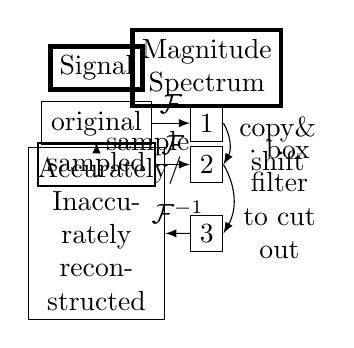
\begin{tikzpicture}[scale=0.7]
				\node[rectangle,draw,ultra thick] (signal) at (-1,1.75) {Signal};
				\node[rectangle,draw,ultra thick,align=center] (magn0) at (1,1.75) {Magnitude\\Spectrum};
				\node[rectangle,draw] (original) at (-1,0.75) {original};
				\node[rectangle,draw,align=center] (magn1) at (1,0.75) {1};
				\node[rectangle,draw,align=center] (sampled) at (-1,0) {sampled};
				\node[rectangle,draw,align=center] (magn2) at (1,0) {2};
				\node[rectangle,draw,align=center,text width=1.5cm] (accorin) at (-1,-1.25) {Accurately/ Inaccurately reconstructed};
				\node[rectangle,draw,align=center] (magn3) at (1,-1.25) {3};
				\path[-latex,draw] (original) to[right] node{sample} (sampled);
				\path[-latex,draw] (original) to[above] node{$\mathcal{F}$} (magn1);
				\path[-latex,draw] (sampled) to[above] node{$\mathcal{F}$} (magn2);
				\path[-latex,draw] (magn1.east) to[bend left,right] node[align=center]{copy\&\\shift} (magn2.east);
				\path[-latex,draw] (magn2.east) to[bend left,right] node[align=center]{$\cdot$ box\\filter\\to cut\\out} (magn3.east);
				\path[-latex,draw] (magn3) to[above] node{$\mathcal{F}^{-1}$} (accorin);
			\end{tikzpicture}
		\end{center}
		In the figure above the accuracy depends on the overlapping wave functions in ``2''. The box filter then can't cut out approprately the magnitude spectrum to get a proper result in ``3''. This leads to an inaccurately reconstructed signal.
	\item[\lp{Proper sampling}] To avoid this effect, this is the procedure: \tikz\node[rectangle,draw] (a) at (0,0) {original signal};$\xrightarrow{\text{lp filtering}}$\tikz\node[rectangle,draw] (a) at (0,0) {lp filt. sign}; $\xrightarrow{\text{sample}}$ \tikz\node[rectangle,draw] (a) at (0,0) {sampl.sign.}; $\xrightarrow{\text{reconstr.}}$ \tikz\node[rectangle,draw] (a) at (0,0) {reconstr.sign};
	\item[\lp{Smoothing as low-pass filtering}] The message of the FT is that high frequencies lead to trouble with sampling.  Solutionsppress high frequencies before sampling.  A filter whose FT is a box is bad, because the filter kernel has infinite support. Common solution: use a Gaussian.
	\item[\lp{Nyquist sampling theorem}]
		Nyquist theorem: The sampling frequency must be at least twice the highest frequency. $\omega_s\geq 2\omega$. If this is no the case, the signal needs to be bandlimited before sampling, e.g. with a low-pass filter.
\section{Image Restoration}
	\item[\lp{Pixelization}]
		Possibilities: Square pixels, Gaussian reconstruction filter, Bilinear interpolation, perfect reconstruction filter.
	\item[\lp{Motion blurring}] Each light dot is transformed into a short line along the $x_1$-axis:
		\begin{gather*}
			h(x_1,x_2)=\frac{1}{2\ell}\left[ \theta(x_1+\ell)-\theta(x_1-\ell) \right]\delta(x_2)
		\end{gather*}
	\item[\lp{Noise}] Gaussian blurring kernel:
		\begin{gather*}
			h(x_1,x_2)=\frac{1}{2\pi\sigma^2}\exp\!\left( -\frac{x_{1}^{2}+x_{2}^{2}}{2\sigma^2} \right)
		\end{gather*}
	\item[\lp{Problem}] $f(\vtr{x})\xrightarrow{\ds h(\vtr{x})}g(\vtr{x})\xrightarrow{\ds\tilde{h}(\vtr{x})}f(\vtr{x})$. The ``inverse'' kernel $\tilde{h}(\vtr{x})$ should compensate the effect of  the image degradation $h(\vtr{x})$, i.e.,
		\begin{gather*}
			\left( \tilde{h}*h \right)(\vtr{x})=\delta(\vtr{x})
		\end{gather*}
		$\tilde{h}(x)$ may be determined more easily in Fourier space:
		\begin{gather*}
			\mathcal{F}\!\left[ \tilde{h} \right]\!(u,v)\cdot\mathcal{F}[h](u,v)=1
		\end{gather*}
		To determine $\mathcal{F}\!\left[ \tilde{h} \right]\!$, we need to estimate
		\begin{inparaenum}[\itshape(1)]
			\item the distortion model $h(\vtr{x})$ (point spread function) or $\mathcal{F}[h](u,v)$ (modulation transfer function)
			\item the parameters of $h(\vtr{x})$, e.g. for defocussing
		\end{inparaenum}
	\item[\lp{Motion Blur FT}] 
		\begin{align*}
			\mathcal{F}[h](u,v)&=\frac{1}{2\ell}{\scriptstyle\int\limits_{-\ell}^{\ell}}\rd x_1\, \exp\!\left( -i2\pi ux_1 \right)\\
			&\quad\cdot\underbrace{{\scriptstyle\int\limits_{-\infty}^{\infty}}\rd x_2\, \delta(x_2)\exp\!\left( -i2\pi vx_2 \right)}_{=1}\\
			&=\sinc\!\left(2\pi u\ell  \right)
		\end{align*}
		Problem: $\mathcal{F}[\tilde{h}](u)=1/\hat{h}(u)$. $\sinc$ has many zeroes and these frequencies can't be recovered! Solution: Regularized reconstruction filter
		\begin{gather*}
			\tilde{F}[\tilde{h}](u,v)=\frac{\mathcal{F}[h]}{\norm{\mathcal{F}}^2+\varepsilon}
		\end{gather*}
		Singularities are avoided by the rugelarization $\varepsilon$.
	\item[\lp{Space-time super-resolution}] One can put two movies of the same thing and merge their frames for space and time super-resolution.
	\item[\lp{Spatial super-resolution}] 
		\begin{inparaitem}
			\item $\text{lens}+\text{pixel}=\text{low-pass filter}$ (edisered to avoid aliasing)
			\item Low-res images $=D*H*G*\text{(desired high-res-image)}$. D:decimate, H:lens+pixel, G: Geometric warp
			\item Smplified case for translation: $LR=(D*G)*(H*HR)$. G is shift-invariant and commutes with H. First compute H HR, then deconvolve HR with H.
			\item Super-resolution needs to restore attenuated frequencies. Many images improve $S/N$ ration $\sim\sqrt{n}$, which helps. Eventually Gaussian's double exponential always dominates.
		\end{inparaitem}
\end{compactdesc}
